\documentclass[12pt,letterpaper]{article}
\usepackage[letterpaper,margin=1in]{geometry}

\usepackage{accsupp}
\usepackage{amsmath}
\usepackage{fontspec}
\usepackage{graphicx}
\usepackage{float}
\usepackage{listings,avrlang}
\usepackage{siunitx}
\usepackage{tikz}
\usepackage{xcolor}

% we dont fw ugly
\setmainfont{Palatino ET W02 Roman}[
	BoldFont=Palatino ET W02 Bold,
	ItalicFont=Palatino ET W02 Italic,
	BoldItalicFont=PalatinoETW02-BoldItali,
	Scale=0.8]
\setmonofont{Courier Prime}[Scale=0.9]

% keep page and line numbers from being selected just in awful case
\renewcommand{\thelstnumber}{\protect\BeginAccSupp{ActualText={}}%
	\arabic{lstnumber}%
\protect\EndAccSupp{}}

\renewcommand{\thepage}{\protect\BeginAccSupp{ActualText={}}%
	\arabic{page}%
\protect\EndAccSupp{}}

% for our beautiful schematic
\usetikzlibrary{
	arrows,
	backgrounds,
	calc,
	fit,
	matrix,
	patterns,
	plotmarks,
	shadows,
	shapes,
	snakes
}

\definecolor{Green}{HTML}{006600}
\definecolor{Blue}{HTML}{2d2f92}
\definecolor{Purple}{HTML}{99479b}
\definecolor{Orange}{HTML}{f58137}
\definecolor{Red}{HTML}{ed1b23}
\lstset{
	language=AVR,
	basicstyle=\small\ttfamily,
	keywordstyle=\color{Blue}\bfseries,
	keywordstyle=[2]\color{Orange},
	keywordstyle=[3]\color{Purple},
	keywordstyle=[4]\color{Red},
	commentstyle=\small\itshape\color{Green},
	tabsize=8,
	numbers=left,
	numberstyle=\small\ttfamily\color{Blue}
}

\title{ECE:3360 -- Lab 2 Report}
\author{Oliver Emery}
\date{23 February 2022}

\begin{document}
\maketitle

\section{Introduction}
The goal of this lab was to construct a simple stopwatch using shift registers,
7-segment displays, and two buttons.
\par The stopwatch must implement two modes with different timer resolutions.
In Mode I, the stopwatch should begin with ``0.0'' displayed. When the first
button is pressed, the display should increment every 0.1 seconds, updating the
display to ``0.1'', ``0.2'', and so on until the display reaches ``9.9''.
Pushing the first button while the stopwatch is counting up should stop the
counter and freeze the display. Pressing the first button while paused should
continue the timer. Once 9.9 seconds have elapsed in Mode I, the display should
flash ``9.9'' once every two seconds. Pressing the second button for less than a
second in any state should stop the counter and reset the stopwatch to 0.
\par In Mode II the stopwatch should function identically to Mode I. However,
the timer should increment in steps of 1 second instead of 0.1 seconds.
Similarly, the stopwatch should now show ``00'' at the start and ``99'' for
overflows.
\par Pressing the second button for more than 1 second should reset the
stopwatch to 0 and alternate between modes I and II.

\section{Schematic}
\begin{figure}[H]
	\centering
	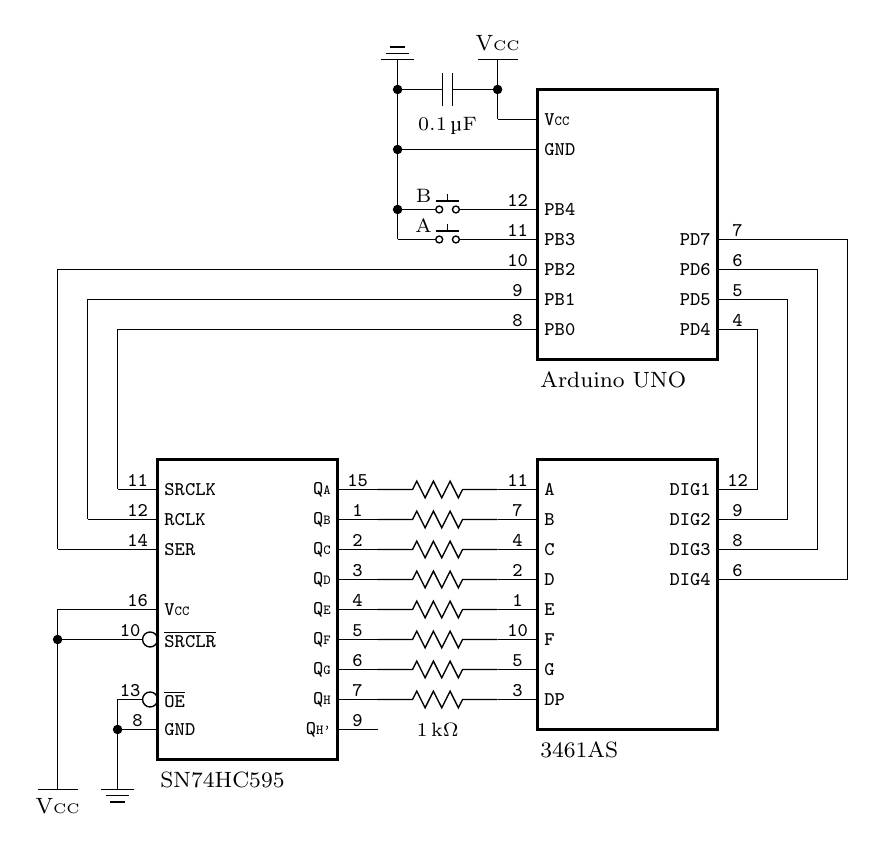
\begin{tikzpicture}[scale=2.54]%
% dpic version 2021.11.01 option -g for TikZ and PGF 1.01
\ifx\dpiclw\undefined\newdimen\dpiclw\fi
\global\def\dpicdraw{\draw[line width=\dpiclw]}
\global\def\dpicstop{;}
\dpiclw=0.8bp
\dpiclw=0.8bp
{\footnotesize
\dpicdraw (0.2,-0.711111) rectangle (1.1,0.788889)\dpicstop
\dpiclw=0.5bp
\draw (0.22,-0.561111) node[right=-2bp]{{\ttfamily\scriptsize GND}};
\dpicdraw (0.2,-0.561111)
 --(-0,-0.561111)\dpicstop
\draw (0.1,-0.561111) node[above=-2bp]{{\ttfamily\scriptsize 8}};
\dpiclw=2bp
\dpiclw=0.5bp
\draw (0.22,-0.411111) node[right=-2bp]{{\ttfamily\scriptsize $\overline{\hbox{OE}}$}};
\dpicdraw (0.1625,-0.411111) circle (0.014764in)\dpicstop
\dpicdraw (0.125,-0.411111)
 --(-0,-0.411111)\dpicstop
\draw (0.0625,-0.411111) node[above=-2bp]{{\ttfamily\scriptsize 13}};
\dpiclw=2bp
\dpiclw=0.5bp
\draw (0.22,-0.111111) node[right=-2bp]{{\ttfamily\scriptsize $\overline{\hbox{SRCLR}}$}};
\dpicdraw (0.1625,-0.111111) circle (0.014764in)\dpicstop
\dpicdraw (0.125,-0.111111)
 --(-0,-0.111111)\dpicstop
\draw (0.0625,-0.111111) node[above=-2bp]{{\ttfamily\scriptsize 10}};
\dpiclw=2bp
\dpiclw=0.5bp
\draw (0.22,0.038889) node[right=-2bp]{{\ttfamily\scriptsize V\hbox{\tiny CC}}};
\dpicdraw (0.2,0.038889)
 --(-0,0.038889)\dpicstop
\draw (0.1,0.038889) node[above=-2bp]{{\ttfamily\scriptsize 16}};
\dpiclw=2bp
\dpiclw=0.5bp
\draw (0.22,0.338889) node[right=-2bp]{{\ttfamily\scriptsize SER}};
\dpicdraw (0.2,0.338889)
 --(-0,0.338889)\dpicstop
\draw (0.1,0.338889) node[above=-2bp]{{\ttfamily\scriptsize 14}};
\dpiclw=2bp
\dpiclw=0.5bp
\draw (0.22,0.488889) node[right=-2bp]{{\ttfamily\scriptsize RCLK}};
\dpicdraw (0.2,0.488889)
 --(-0,0.488889)\dpicstop
\draw (0.1,0.488889) node[above=-2bp]{{\ttfamily\scriptsize 12}};
\dpiclw=2bp
\dpiclw=0.5bp
\draw (0.22,0.638889) node[right=-2bp]{{\ttfamily\scriptsize SRCLK}};
\dpicdraw (0.2,0.638889)
 --(-0,0.638889)\dpicstop
\draw (0.1,0.638889) node[above=-2bp]{{\ttfamily\scriptsize 11}};
\dpiclw=2bp
\dpiclw=0.5bp
\draw (1.08,-0.561111) node[left=-2bp]{{\ttfamily\scriptsize Q\hbox{\tiny H\rq}}};
\dpicdraw (1.1,-0.561111)
 --(1.3,-0.561111)\dpicstop
\draw (1.2,-0.561111) node[above=-2bp]{{\ttfamily\scriptsize 9}};
\dpiclw=2bp
\dpiclw=0.5bp
\draw (1.08,-0.411111) node[left=-2bp]{{\ttfamily\scriptsize Q\hbox{\tiny H}}};
\dpicdraw (1.1,-0.411111)
 --(1.3,-0.411111)\dpicstop
\draw (1.2,-0.411111) node[above=-2bp]{{\ttfamily\scriptsize 7}};
\dpiclw=2bp
\dpiclw=0.5bp
\draw (1.08,-0.261111) node[left=-2bp]{{\ttfamily\scriptsize Q\hbox{\tiny G}}};
\dpicdraw (1.1,-0.261111)
 --(1.3,-0.261111)\dpicstop
\draw (1.2,-0.261111) node[above=-2bp]{{\ttfamily\scriptsize 6}};
\dpiclw=2bp
\dpiclw=0.5bp
\draw (1.08,-0.111111) node[left=-2bp]{{\ttfamily\scriptsize Q\hbox{\tiny F}}};
\dpicdraw (1.1,-0.111111)
 --(1.3,-0.111111)\dpicstop
\draw (1.2,-0.111111) node[above=-2bp]{{\ttfamily\scriptsize 5}};
\dpiclw=2bp
\dpiclw=0.5bp
\draw (1.08,0.038889) node[left=-2bp]{{\ttfamily\scriptsize Q\hbox{\tiny E}}};
\dpicdraw (1.1,0.038889)
 --(1.3,0.038889)\dpicstop
\draw (1.2,0.038889) node[above=-2bp]{{\ttfamily\scriptsize 4}};
\dpiclw=2bp
\dpiclw=0.5bp
\draw (1.08,0.188889) node[left=-2bp]{{\ttfamily\scriptsize Q\hbox{\tiny D}}};
\dpicdraw (1.1,0.188889)
 --(1.3,0.188889)\dpicstop
\draw (1.2,0.188889) node[above=-2bp]{{\ttfamily\scriptsize 3}};
\dpiclw=2bp
\dpiclw=0.5bp
\draw (1.08,0.338889) node[left=-2bp]{{\ttfamily\scriptsize Q\hbox{\tiny C}}};
\dpicdraw (1.1,0.338889)
 --(1.3,0.338889)\dpicstop
\draw (1.2,0.338889) node[above=-2bp]{{\ttfamily\scriptsize 2}};
\dpiclw=2bp
\dpiclw=0.5bp
\draw (1.08,0.488889) node[left=-2bp]{{\ttfamily\scriptsize Q\hbox{\tiny B}}};
\dpicdraw (1.1,0.488889)
 --(1.3,0.488889)\dpicstop
\draw (1.2,0.488889) node[above=-2bp]{{\ttfamily\scriptsize 1}};
\dpiclw=2bp
\dpiclw=0.5bp
\draw (1.08,0.638889) node[left=-2bp]{{\ttfamily\scriptsize Q\hbox{\tiny A}}};
\dpicdraw (1.1,0.638889)
 --(1.3,0.638889)\dpicstop
\draw (1.2,0.638889) node[above=-2bp]{{\ttfamily\scriptsize 15}};
\dpiclw=2bp
\draw (0.2,-0.761111) node[below right=-2bp]{SN74HC595};
\dpiclw=0.8bp
\dpicdraw (2.1,-0.561111) rectangle (3,0.788889)\dpicstop
\dpiclw=0.5bp
\draw (2.12,-0.411111) node[right=-2bp]{{\ttfamily\scriptsize DP}};
\dpicdraw (2.1,-0.411111)
 --(1.9,-0.411111)\dpicstop
\draw (2,-0.411111) node[above=-2bp]{{\ttfamily\scriptsize 3}};
\dpiclw=2bp
\dpiclw=0.5bp
\draw (2.12,-0.261111) node[right=-2bp]{{\ttfamily\scriptsize G}};
\dpicdraw (2.1,-0.261111)
 --(1.9,-0.261111)\dpicstop
\draw (2,-0.261111) node[above=-2bp]{{\ttfamily\scriptsize 5}};
\dpiclw=2bp
\dpiclw=0.5bp
\draw (2.12,-0.111111) node[right=-2bp]{{\ttfamily\scriptsize F}};
\dpicdraw (2.1,-0.111111)
 --(1.9,-0.111111)\dpicstop
\draw (2,-0.111111) node[above=-2bp]{{\ttfamily\scriptsize 10}};
\dpiclw=2bp
\dpiclw=0.5bp
\draw (2.12,0.038889) node[right=-2bp]{{\ttfamily\scriptsize E}};
\dpicdraw (2.1,0.038889)
 --(1.9,0.038889)\dpicstop
\draw (2,0.038889) node[above=-2bp]{{\ttfamily\scriptsize 1}};
\dpiclw=2bp
\dpiclw=0.5bp
\draw (2.12,0.188889) node[right=-2bp]{{\ttfamily\scriptsize D}};
\dpicdraw (2.1,0.188889)
 --(1.9,0.188889)\dpicstop
\draw (2,0.188889) node[above=-2bp]{{\ttfamily\scriptsize 2}};
\dpiclw=2bp
\dpiclw=0.5bp
\draw (2.12,0.338889) node[right=-2bp]{{\ttfamily\scriptsize C}};
\dpicdraw (2.1,0.338889)
 --(1.9,0.338889)\dpicstop
\draw (2,0.338889) node[above=-2bp]{{\ttfamily\scriptsize 4}};
\dpiclw=2bp
\dpiclw=0.5bp
\draw (2.12,0.488889) node[right=-2bp]{{\ttfamily\scriptsize B}};
\dpicdraw (2.1,0.488889)
 --(1.9,0.488889)\dpicstop
\draw (2,0.488889) node[above=-2bp]{{\ttfamily\scriptsize 7}};
\dpiclw=2bp
\dpiclw=0.5bp
\draw (2.12,0.638889) node[right=-2bp]{{\ttfamily\scriptsize A}};
\dpicdraw (2.1,0.638889)
 --(1.9,0.638889)\dpicstop
\draw (2,0.638889) node[above=-2bp]{{\ttfamily\scriptsize 11}};
\dpiclw=2bp
\dpiclw=0.5bp
\draw (2.98,0.188889) node[left=-2bp]{{\ttfamily\scriptsize DIG4}};
\dpicdraw (3,0.188889)
 --(3.2,0.188889)\dpicstop
\draw (3.1,0.188889) node[above=-2bp]{{\ttfamily\scriptsize 6}};
\dpiclw=2bp
\dpiclw=0.5bp
\draw (2.98,0.338889) node[left=-2bp]{{\ttfamily\scriptsize DIG3}};
\dpicdraw (3,0.338889)
 --(3.2,0.338889)\dpicstop
\draw (3.1,0.338889) node[above=-2bp]{{\ttfamily\scriptsize 8}};
\dpiclw=2bp
\dpiclw=0.5bp
\draw (2.98,0.488889) node[left=-2bp]{{\ttfamily\scriptsize DIG2}};
\dpicdraw (3,0.488889)
 --(3.2,0.488889)\dpicstop
\draw (3.1,0.488889) node[above=-2bp]{{\ttfamily\scriptsize 9}};
\dpiclw=2bp
\dpiclw=0.5bp
\draw (2.98,0.638889) node[left=-2bp]{{\ttfamily\scriptsize DIG1}};
\dpicdraw (3,0.638889)
 --(3.2,0.638889)\dpicstop
\draw (3.1,0.638889) node[above=-2bp]{{\ttfamily\scriptsize 12}};
\dpiclw=2bp
\draw (2.1,-0.611111) node[below right=-2bp]{3461AS};
\dpiclw=0.8bp
\dpicdraw (2.1,1.288889) rectangle (3,2.638889)\dpicstop
\dpiclw=0.5bp
\draw (2.12,1.438889) node[right=-2bp]{{\ttfamily\scriptsize PB0}};
\dpicdraw (2.1,1.438889)
 --(1.9,1.438889)\dpicstop
\draw (2,1.438889) node[above=-2bp]{{\ttfamily\scriptsize 8}};
\dpiclw=2bp
\dpiclw=0.5bp
\draw (2.12,1.588889) node[right=-2bp]{{\ttfamily\scriptsize PB1}};
\dpicdraw (2.1,1.588889)
 --(1.9,1.588889)\dpicstop
\draw (2,1.588889) node[above=-2bp]{{\ttfamily\scriptsize 9}};
\dpiclw=2bp
\dpiclw=0.5bp
\draw (2.12,1.738889) node[right=-2bp]{{\ttfamily\scriptsize PB2}};
\dpicdraw (2.1,1.738889)
 --(1.9,1.738889)\dpicstop
\draw (2,1.738889) node[above=-2bp]{{\ttfamily\scriptsize 10}};
\dpiclw=2bp
\dpiclw=0.5bp
\draw (2.12,1.888889) node[right=-2bp]{{\ttfamily\scriptsize PB3}};
\dpicdraw (2.1,1.888889)
 --(1.9,1.888889)\dpicstop
\draw (2,1.888889) node[above=-2bp]{{\ttfamily\scriptsize 11}};
\dpiclw=2bp
\dpiclw=0.5bp
\draw (2.12,2.038889) node[right=-2bp]{{\ttfamily\scriptsize PB4}};
\dpicdraw (2.1,2.038889)
 --(1.9,2.038889)\dpicstop
\draw (2,2.038889) node[above=-2bp]{{\ttfamily\scriptsize 12}};
\dpiclw=2bp
\dpiclw=0.5bp
\draw (2.12,2.338889) node[right=-2bp]{{\ttfamily\scriptsize GND}};
\dpicdraw (2.1,2.338889)
 --(1.9,2.338889)\dpicstop
\dpiclw=2bp
\dpiclw=0.5bp
\draw (2.12,2.488889) node[right=-2bp]{{\ttfamily\scriptsize V\hbox{\tiny CC}}};
\dpicdraw (2.1,2.488889)
 --(1.9,2.488889)\dpicstop
\dpiclw=2bp
\dpiclw=0.5bp
\draw (2.98,1.438889) node[left=-2bp]{{\ttfamily\scriptsize PD4}};
\dpicdraw (3,1.438889)
 --(3.2,1.438889)\dpicstop
\draw (3.1,1.438889) node[above=-2bp]{{\ttfamily\scriptsize 4}};
\dpiclw=2bp
\dpiclw=0.5bp
\draw (2.98,1.588889) node[left=-2bp]{{\ttfamily\scriptsize PD5}};
\dpicdraw (3,1.588889)
 --(3.2,1.588889)\dpicstop
\draw (3.1,1.588889) node[above=-2bp]{{\ttfamily\scriptsize 5}};
\dpiclw=2bp
\dpiclw=0.5bp
\draw (2.98,1.738889) node[left=-2bp]{{\ttfamily\scriptsize PD6}};
\dpicdraw (3,1.738889)
 --(3.2,1.738889)\dpicstop
\draw (3.1,1.738889) node[above=-2bp]{{\ttfamily\scriptsize 6}};
\dpiclw=2bp
\dpiclw=0.5bp
\draw (2.98,1.888889) node[left=-2bp]{{\ttfamily\scriptsize PD7}};
\dpicdraw (3,1.888889)
 --(3.2,1.888889)\dpicstop
\draw (3.1,1.888889) node[above=-2bp]{{\ttfamily\scriptsize 7}};
\dpiclw=2bp
\draw (2.1,1.238889) node[below right=-2bp]{Arduino UNO};
\dpiclw=0.8bp
\dpiclw=0.5bp
\dpicdraw (1.3,0.638889)
 --(1.475,0.638889)
 --(1.495833,0.680556)
 --(1.5375,0.597222)
 --(1.579167,0.680556)
 --(1.620833,0.597222)
 --(1.6625,0.680556)
 --(1.704167,0.597222)
 --(1.725,0.638889)
 --(1.9,0.638889)\dpicstop
\dpicdraw (1.3,0.488889)
 --(1.475,0.488889)
 --(1.495833,0.530556)
 --(1.5375,0.447222)
 --(1.579167,0.530556)
 --(1.620833,0.447222)
 --(1.6625,0.530556)
 --(1.704167,0.447222)
 --(1.725,0.488889)
 --(1.9,0.488889)\dpicstop
\dpicdraw (1.3,0.338889)
 --(1.475,0.338889)
 --(1.495833,0.380556)
 --(1.5375,0.297222)
 --(1.579167,0.380556)
 --(1.620833,0.297222)
 --(1.6625,0.380556)
 --(1.704167,0.297222)
 --(1.725,0.338889)
 --(1.9,0.338889)\dpicstop
\dpicdraw (1.3,0.188889)
 --(1.475,0.188889)
 --(1.495833,0.230556)
 --(1.5375,0.147222)
 --(1.579167,0.230556)
 --(1.620833,0.147222)
 --(1.6625,0.230556)
 --(1.704167,0.147222)
 --(1.725,0.188889)
 --(1.9,0.188889)\dpicstop
\dpicdraw (1.3,0.038889)
 --(1.475,0.038889)
 --(1.495833,0.080556)
 --(1.5375,-0.002778)
 --(1.579167,0.080556)
 --(1.620833,-0.002778)
 --(1.6625,0.080556)
 --(1.704167,-0.002778)
 --(1.725,0.038889)
 --(1.9,0.038889)\dpicstop
\dpicdraw (1.3,-0.111111)
 --(1.475,-0.111111)
 --(1.495833,-0.069444)
 --(1.5375,-0.152778)
 --(1.579167,-0.069444)
 --(1.620833,-0.152778)
 --(1.6625,-0.069444)
 --(1.704167,-0.152778)
 --(1.725,-0.111111)
 --(1.9,-0.111111)\dpicstop
\dpicdraw (1.3,-0.261111)
 --(1.475,-0.261111)
 --(1.495833,-0.219444)
 --(1.5375,-0.302778)
 --(1.579167,-0.219444)
 --(1.620833,-0.302778)
 --(1.6625,-0.219444)
 --(1.704167,-0.302778)
 --(1.725,-0.261111)
 --(1.9,-0.261111)\dpicstop
\dpicdraw (1.3,-0.411111)
 --(1.475,-0.411111)
 --(1.495833,-0.369444)
 --(1.5375,-0.452778)
 --(1.579167,-0.369444)
 --(1.620833,-0.452778)
 --(1.6625,-0.369444)
 --(1.704167,-0.452778)
 --(1.725,-0.411111)
 --(1.9,-0.411111)\dpicstop
\draw (1.6,-0.561111) node{\scriptsize \SI{1}{\kilo\ohm}};
\dpicdraw (0,-0.411111)
 --(0,-0.861111)\dpicstop
\dpicdraw (0.083333,-0.861111)
 --(-0.083333,-0.861111)\dpicstop
\dpicdraw (0.055556,-0.892361)
 --(-0.055556,-0.892361)\dpicstop
\dpicdraw (0.035714,-0.923611)
 --(-0.035714,-0.923611)\dpicstop
\dpicdraw[fill=black](-0,-0.561111) circle (0.007874in)\dpicstop
\dpicdraw (3.2,1.438889)
 --(3.2,0.638889)\dpicstop
\dpicdraw (3.2,1.588889)
 --(3.35,1.588889)\dpicstop
\dpicdraw (3.35,1.588889)
 --(3.35,0.488889)\dpicstop
\dpicdraw (3.35,0.488889)
 --(3.2,0.488889)\dpicstop
\dpicdraw (3.2,1.738889)
 --(3.5,1.738889)\dpicstop
\dpicdraw (3.5,1.738889)
 --(3.5,0.338889)\dpicstop
\dpicdraw (3.5,0.338889)
 --(3.2,0.338889)\dpicstop
\dpicdraw (3.2,1.888889)
 --(3.65,1.888889)\dpicstop
\dpicdraw (3.65,1.888889)
 --(3.65,0.188889)\dpicstop
\dpicdraw (3.65,0.188889)
 --(3.2,0.188889)\dpicstop
\dpicdraw (1.9,1.438889)
 --(0,1.438889)\dpicstop
\dpicdraw (0,1.438889)
 --(-0,0.638889)\dpicstop
\dpicdraw (1.9,1.588889)
 --(-0.15,1.588889)\dpicstop
\dpicdraw (-0.15,1.588889)
 --(-0.15,0.488889)\dpicstop
\dpicdraw (-0.15,0.488889)
 --(-0,0.488889)\dpicstop
\dpicdraw (1.9,1.738889)
 --(-0.3,1.738889)\dpicstop
\dpicdraw (-0.3,1.738889)
 --(-0.3,0.338889)\dpicstop
\dpicdraw (-0.3,0.338889)
 --(-0,0.338889)\dpicstop
\dpicdraw (1.4,1.888889)
 --(1.591037,1.888889)\dpicstop
\dpicdraw (1.608333,1.888889) circle (0.00681in)\dpicstop
\dpicdraw (1.691667,1.888889) circle (0.00681in)\dpicstop
\dpicdraw (1.591037,1.93213)
 --(1.708963,1.93213)\dpicstop
\dpicdraw (1.65,1.93213)
 --(1.65,1.966723)\dpicstop
\dpicdraw (1.708963,1.888889)
 --(1.9,1.888889)\dpicstop
\dpicdraw (1.4,2.038889)
 --(1.591037,2.038889)\dpicstop
\dpicdraw (1.608333,2.038889) circle (0.00681in)\dpicstop
\dpicdraw (1.691667,2.038889) circle (0.00681in)\dpicstop
\dpicdraw (1.591037,2.08213)
 --(1.708963,2.08213)\dpicstop
\dpicdraw (1.65,2.08213)
 --(1.65,2.116723)\dpicstop
\dpicdraw (1.708963,2.038889)
 --(1.9,2.038889)\dpicstop
\dpicdraw (1.9,2.338889)
 --(1.4,2.338889)\dpicstop
\dpicdraw (1.4,1.888889)
 --(1.4,2.788889)\dpicstop
\dpicdraw (1.316667,2.788889)
 --(1.483333,2.788889)\dpicstop
\dpicdraw (1.344444,2.820139)
 --(1.455556,2.820139)\dpicstop
\dpicdraw (1.364286,2.851389)
 --(1.435714,2.851389)\dpicstop
\dpicdraw[fill=black](1.4,2.038889) circle (0.007874in)\dpicstop
\dpicdraw[fill=black](1.4,2.338889) circle (0.007874in)\dpicstop
\dpicdraw (1.9,2.488889)
 --(1.9,2.788889)\dpicstop
\draw (1.9,2.818889) node[above=-2bp]{V\hbox{\tiny CC}};
\dpicdraw (1.8,2.788889)
 --(2,2.788889)\dpicstop
\dpicdraw (1.4,2.638889)
 --(1.625,2.638889)\dpicstop
\dpicdraw (1.625,2.555556)
 --(1.625,2.722222)\dpicstop
\dpicdraw (1.675,2.555556)
 --(1.675,2.722222)\dpicstop
\dpicdraw (1.675,2.638889)
 --(1.9,2.638889)\dpicstop
\draw (1.65,2.458889) node{\scriptsize\SI{0.1}{\micro\farad}};
\dpicdraw[fill=black](1.4,2.638889) circle (0.007874in)\dpicstop
\dpicdraw[fill=black](1.9,2.638889) circle (0.007874in)\dpicstop
\dpicdraw (0,-0.111111)
 --(-0.3,-0.111111)\dpicstop
\dpicdraw (-0,0.038889)
 --(-0.3,0.038889)\dpicstop
\dpicdraw (-0.3,0.038889)
 --(-0.3,-0.861111)\dpicstop
\draw (-0.3,-0.891111) node[below=-2bp]{V\hbox{\tiny CC}};
\dpicdraw (-0.4,-0.861111)
 --(-0.2,-0.861111)\dpicstop
\dpicdraw[fill=black](-0.3,-0.111111) circle (0.007874in)\dpicstop
\draw (1.53,2.108889) node{{\scriptsize B}};
\draw (1.53,1.958889) node{{\scriptsize A}};
}
\end{tikzpicture}%

	\caption{schematic as implemented}
\end{figure}
\begin{figure}[H]
	\centering
	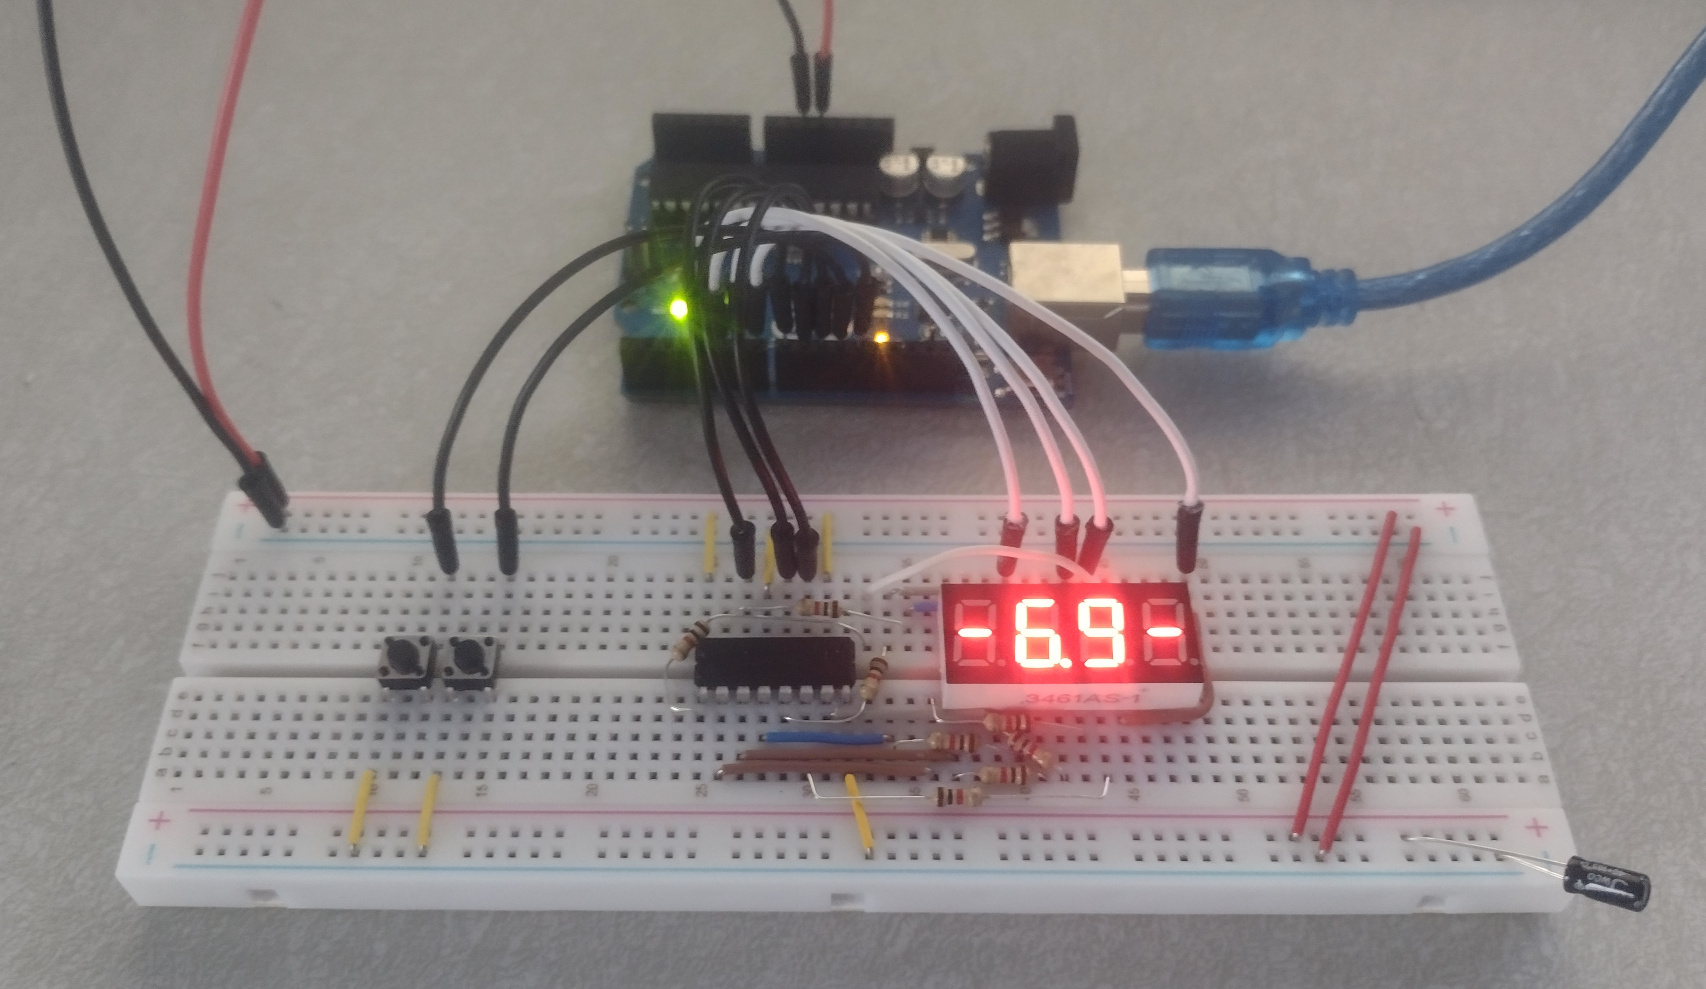
\includegraphics[width=0.8\textwidth]{images/implementation.jpg}
	\caption{physical implementation}
\end{figure}

\section{Discussion}
I used \SI{1}{\kilo\ohm} resistors for the seven-segment display
in order to keep the current through each segment well beneath the target value
of \SI{6}{mA}. I also included a standard \SI{0.1}{\micro\farad} decoupling
capacitor to smooth ripples in the power supply.

\subsection{Hardware Design}
The final design was almost identical to that prescribed in the lab manual, with
the exception of the four-digit display. Fortunately, the pinout of the 3461AS
was nearly identical to that of the 5161AS, and only required one additional
wire for each digit.

\subsection{Buttons and Debouncing}
Each button has an associated structure in SRAM containing relevant information.
I aimed to keep the debouncing logic as simple as possible: register a change
in button state if and only if it maintains that changed state over a minimum
period of time. An unregistered change occurs when the button state in memory
differs from the button's hardware state. The final implementation requires
50 stable samples at \SI{1}{ms} intervals to register a change.
\par Also included in the button structure is a duration field, incremented
every \SI{100}{ms} when a button is in the pressed state. This value is used
when button B is released to determine whether or not to change the mode.

\subsection{Four-digit Seven-segment Display}
\par In pursuit of extra credit, I created the design with a four-digit
seven-sigment display. The 3461AS can only display one unique digit at a time,
with power controlled by one pin for each digit. One study\footnotemark[1]
found that humans can detect flicker at an extreme of \SI{500}{Hz}. With a
system clock of \SI{16}{MHz}, a refresh rate as large as \SI{1}{KHz} still
affords an entire 16,000 cycles to spend per refresh. For each refresh, the
stopwatch must display each digit for a distinct but equal period of time.
\par The shift register supports clock speeds up to \SI{20}{MHz}; the final
implementation requires approximately \SI{8}{\micro\second} (lines 574-634) to
shift one byte into the shift register. No display digit is powered while the shift
register is loaded. In order to maximize the duty cycle of each digit, it is
ideal for each digit to be powered substantially longer than it is not during
its 25\% of each refresh. Lines 635-648 below produce a delay of approximately
\SI{48}{\micro\second}, resulting in a final duty cycle of \[
	25\% \cdot \frac{48}{8+48}\approx 21.4\%
\] for each digit. Unsurprisingly, reducing the duty cycle dims the digits.
Each refresh in the final implementation takes approximately
\SI{230}{\micro\second} (lines 576-611), which corresponds to a refresh rate of
\SI{4.35}{kHz}. Indeed, no flicker is detectable with the naked eye.
\par To control power to the display digits, one I/O pin is assigned to each of
the four digits. While this method is simple and convenient, it would also be
feasible to use another shift register in lieu of I/O pins to control power to
each digit. While this would increase I/O pin availability, it would increase
hardware cost and increase code complexity {\footnotesize marginally}.
\footnotetext[1]{https://www.nature.com/articles/srep07861}
\par See source comments in Appendix A for more local and detailed discussion.

\newpage\appendix
\section{Source Code Listing}
\lstinputlisting{main.S}

\end{document}
